\subsection{Test Results}
The results of the unit test should be included in the documentation.  The results can be discussed verbally, but also included as tables and figures.  

\subsection{Unit Test Table Results}
To automatically create a unit test table to include in the documentation, use the command:
\begin{verbatim}
unitTestSupport.writeTableLaTeX(
tableName,
tableHeaders,
caption,
dataMatrix,
path)
\end{verbatim}
%Here {\tt tableName} is a unique table name that is used to specify the \TeX\ filename and the table reference label.  The array {\tt tableHeaders} contains the column header titles.  Note that these labels can include math variables as well.  The table data is given in the array {\tt dataMatrix}.   This function creates the \TeX\ code for each table, and stores the result inside the documentation folder's {\tt Tables} sub-folder.  For example, the tables \ref{tbl:test11}--\ref{tbl:test22} are auto-generated by the python unit test.  
%
%\begin{table}[htbp]
\caption{Sample output table for param1 = 1 and param2 = 1.}
\label{tbl:test11}
\centering
\begin{tabular}{ccccccc}
\hline
  time [s]  &  Output 1  &  Error  &  Output 2  &  Error  &  Output 3 $\bm r$  &  Error  \\
\hline
     0      &     2      &    0    &     1      &    0    &        0.7         &    0    \\
    0.5     &     3      &    0    &     1      &    0    &        0.7         &    0    \\
     1      &     4      &    0    &     1      &    0    &        0.7         &    0    \\
    1.5     &     2      &    0    &     1      &    0    &        0.7         &    0    \\
     2      &     3      &    0    &     1      &    0    &        0.7         &    0    \\
\hline
\end{tabular}\end{table}
%\begin{table}[htbp]
\caption{Sample output table for param1 = 1 and param2 = 3.}
\label{tbl:test13}
\centering
\begin{tabular}{ccccccc}
\hline
  time [s]  &  Output 1  &  Error  &  Output 2  &  Error  &  Output 3 $\bm r$  &  Error  \\
\hline
     0      &     2      &    0    &     3      &    0    &        0.7         &    0    \\
    0.5     &     3      &    0    &     3      &    0    &        0.7         &    0    \\
     1      &     4      &    0    &     3      &    0    &        0.7         &    0    \\
    1.5     &     2      &    0    &     3      &    0    &        0.7         &    0    \\
     2      &     3      &    0    &     3      &    0    &        0.7         &    0    \\
\hline
\end{tabular}\end{table}
%\begin{table}[htbp]
\caption{Sample output table for param1 = 2 and param2 = 2.}
\label{tbl:test22}
\centering
\begin{tabular}{ccccccc}
\hline
  time [s]  &  Output 1  &  Error  &  Output 2  &  Error  &  Output 3 $\bm r$  &  Error  \\
\hline
     0      &     3      &    0    &     2      &    0    &        0.7         &    0    \\
    0.5     &     4      &    0    &     2      &    0    &        0.7         &    0    \\
     1      &     5      &    0    &     2      &    0    &        0.7         &    0    \\
    1.5     &     3      &    0    &     2      &    0    &        0.7         &    0    \\
     2      &     4      &    0    &     2      &    0    &        0.7         &    0    \\
\hline
\end{tabular}\end{table}


\subsection{Unit Test Figure Results}
If figures and plots are generated in the python unit tests, these can be also automatically included in the unit test documentation.  This is achieved with the command:
\begin{verbatim}
unitTestSupport.writeFigureLaTeX(
"testPlot",
"Illustration of Sample Plot",
plt,
"width=0.5\\textwidth",
path)
\end{verbatim}

%An example of such an automatic inclusion is shown in Figure~\ref{fig:testPlot}.  The figure name is the file name to include, but also the label name to use to reference the figure.  Not that in this figure 3 simulation results are shown in one figure.  These can also be saved off to separate figures if needed.

%\begin{figure}[htbp]
\centerline{
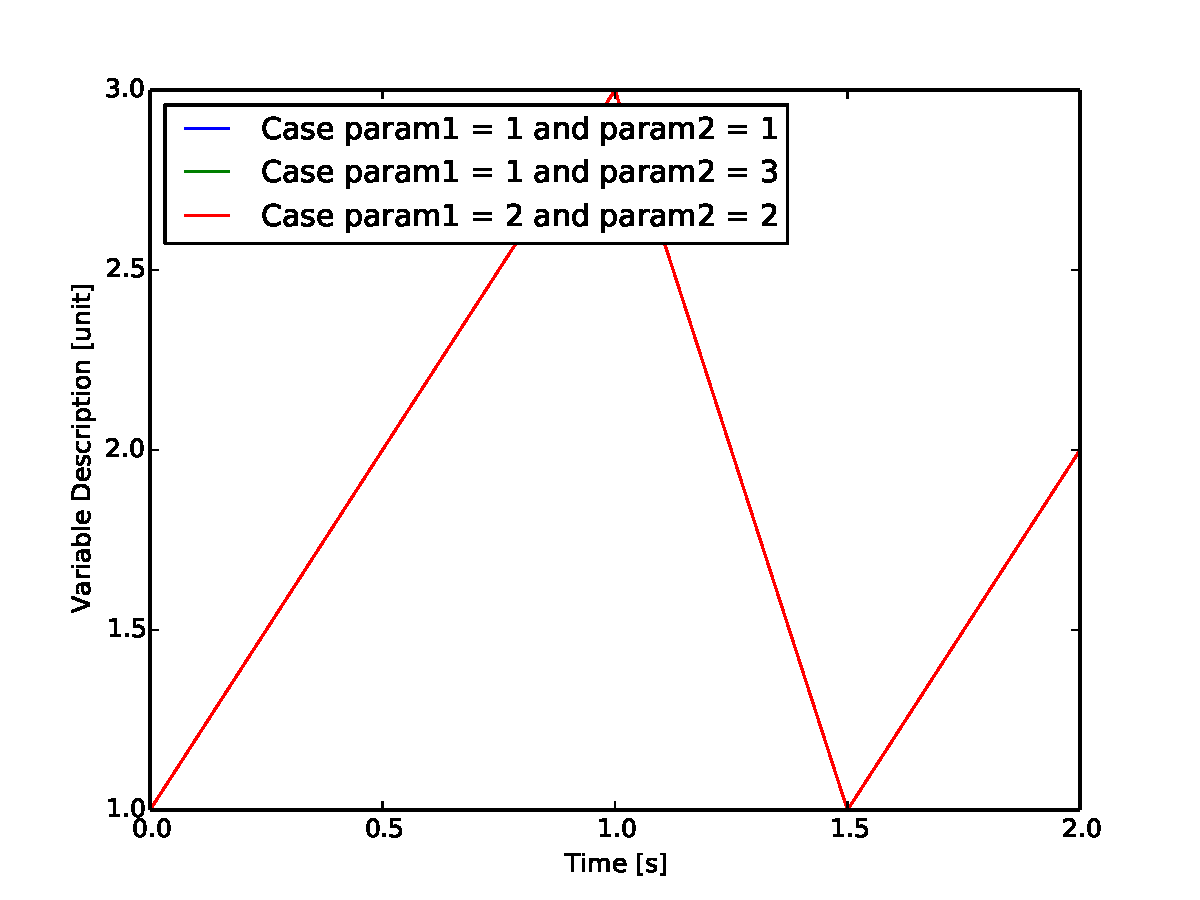
\includegraphics[width=0.5\textwidth]{Figures/testPlot}}
\caption{Illustration of Sample Plot}
\label{fig:testPlot}
\end{figure}

